\documentclass[11pt,a4paper,titlepage,openany]{report}
\usepackage[utf8]{inputenc}
\usepackage[T1]{fontenc}
\usepackage[french]{babel}
\usepackage[top=1.5cm, bottom=4cm]{geometry}
\usepackage{fancyhdr, graphicx, array, hyperref}
\usepackage{glossaries}
%\usepackage{pdfpages}

\pagestyle{fancy}

\title{\textsc{\textbf{Plan projet\\Interpréteur du langage LIR}}}
\date{}
\author{Nicolas \textsc{Caminade} \and Sylvan \textsc{Courtiol} \and
    Pierre \textsc{Debas} \and Heïa \textsc{Dexter} \and Lucàs
    \textsc{Vabre} }
\begin{document}
    \lhead{\leftmark}
    \rhead{
        
\includegraphics[width=2cm]{img/logoiut}
    }

    \cfoot{\thepage}
    \headheight = 2cm
    \headsep = 0.5cm

    \begin{titlepage}
        \fontfamily{pag}\selectfont

        \begin{center}\normalsize
            \MakeUppercase{IUT de Rodez \hfill Département informatique
                \hfill INFO1 2020-2021}
        \end{center}
        \vspace*{0.1cm}
        \hrule
        \vspace*{0.2cm}
        \begin{flushright}
            
\includegraphics[width=4cm]{img/logoiut}
        \end{flushright}
        \vspace*{2cm}
        \begin{flushright}\Huge
            \textsc{\textbf{Plan projet\\Interpréteur du langage LIR}}
        \end{flushright}
        \hrule
        \begin{flushleft}
            \MakeUppercase{Projet proposé par Frédérique Barrios}
        \end{flushleft}
        \vspace*{2cm}
        \begin{center}\Large
            Nicolas \textsc{Caminade}, Sylvan \textsc{Courtiol},\\
            Pierre \textsc{Debas}, Heïa \textsc{Dexter}, \\
            Lucàs \textsc{Vabre}
        \end{center}
        \vfill
        \begin{center}\normalsize
            \MakeUppercase{Projet tuteuré --- Semestre 2}
        \end{center}
    \end{titlepage}

    \renewcommand\rmdefault{pag}
    \fontfamily{pag}\selectfont
    \renewcommand{\sfdefault}{pag}

    % Sommaire
    \renewcommand{\contentsname}{Sommaire}
    \tableofcontents

    \part{Plan projet}

    \chapter*{Introduction}
    \Large
    Dans le cadre des projets tuteuré du semestre 2 de première année de
    DUT informatique de l’année 2020-2021, le sujet de l’Interpréteur LIR
    a été proposé par F. Barrios, un des enseignants de l’IUT de Rodez.
    \\Ce document a pour but de rassembler les informations fondamentales
    relatives à la gestion du projet. Ce plan projet est un document de
    référence du projet qui sera complété tout au long de son avancement.

    \normalsize
    \chapter{Présentation du projet}
    \section{Définition générale du besoin : l'Interpréteur LIR}
    L’Interpréteur LIR est un interpréteur d’un langage de programmation
    simple, il sera nommé LIR pour Langage IUT de Rodez.
    Un interpréteur est un automate enchaînant les tâches suivantes :
    analyse lexico-syntaxique d’une ligne de commande puis interprétation.
    \\Une ligne entrée par un utilisateur sera donc : soit une commande à
    exécuter immédiatement, soit une ligne de programme à mémoriser pour
    une exécution ultérieure. Une ligne de programme se distinguera d'une
    ligne de commande par le fait qu'elle sera toujours précédée d'un
    "numéro d'ordre" appelé aussi "étiquette".

    \section{Cahier des charges}
    Le document en annexe fourni par la maîtrise d’ouvrage (MOA) définit
    l’interpréteur attendu avec les éléments du Langage IUT de Rodez, la
    syntaxe des instructions de programmation et des commandes générales
    attendues dans le logiciel final. Le document précise également le
    comportement attendu de l’interpréteur lors de son utilisation suivi
    d’un exemple d’une session sous cet interpréteur LIR.

    \section{Définitions et acronymes}
        \paragraph{Analyse syntaxique :}
        La vérification de la conformité aux contraintes syntaxiques
        définies par une grammaire.

        \paragraph{Analyse lexicale :}
        L’identification des éléments du vocabulaire d’un langage dans
        une description textuelle (scanning) et la recherche des unités
        lexicales (lexèmes).

        \paragraph{Grammaire :}
        Contraintes syntaxiques définissant les constructions correctes
        (autorisées) d’un langage.

        \paragraph{Interpréteur :}
        Programme capable d’analyser les instructions d’un langage
        (évolué) et de les exécuter directement.

        \paragraph{Langage :}
        Outil de description et d’expression.

        \paragraph{Langage IUT de Rodez (LIR)}

        \paragraph{Sémantique :}
        Étude du sens des unités linguistiques et de leurs combinaisons.
        \\Aspect de la logique qui traite de l'interprétation et de la
        signification des systèmes formels, par opposition à la syntaxe, entendue
        comme l'étude des relations formelles entre formules de tels systèmes
        (d’après le dictionnaire Larousse).

        \paragraph{Syntaxe :}
        Partie de la grammaire qui décrit les règles par lesquelles les unités
        linguistiques se combinent en phrases. En logique, étude des relations
        formelles entre expressions d'un langage (d’après le dictionnaire
        Larousse).
        \\Aussi, la syntaxe est spécifiée par des grammaires et des notations
        formelles.

        \paragraph{Vocabulaire :}
        Symboles de base utilisés dans un langage.

    \section{Charte de projet}
    \subsection{Objectifs du projet}
    Réaliser un interpréteur capable d'exécuter un script ou une série
    d'instructions dans le langage LIR avec les outils et connaissances
    et mis à disposition par l’IUT de Rodez.

    \subsection{Périmètre du projet}
    Ce projet est doit être mené jusqu'à obtention d’un interpréteur
    capable d’exécuter toutes les commandes précisées dans le cahier des
    charges fourni.

    \subsection{Demandes hors périmètre}
    Il n’y a pas de demandes hors périmètre.

    \subsection{Principaux livrables identifiés}
    \paragraph{Livrables :} plan projet, dossier de projet, CD (de
    préférence un dossier compressé plutôt qu’un CD) contenant les codes
    exécutables les fichiers de données, les codes sources et la version
    numérique du dossier et le manuel utilisateur.

    \paragraph{Définition du cadre}
    \subparagraph{Coût :} À définir par le chef de projet (P. Debas).
    \subparagraph{Délais :} Deux dates butoirs identifiées.
        \begin{itemize}
            \item Remise du projet le vendredi 28 mai 2021.
            \item Soutenance du projet la semaine du 7 juin 2021.
        \end{itemize}

    \subparagraph{Qualité :}
    Projet codé en Java dans les respects des conventions et bonnes
    pratiques.

    \subsection{Les acteurs du projet}

    \begin{center}
        \begin{tabular}{rl}
            L'équipe MOE :        & N. CAMINADE, S. COURTIOL, \\
                                  & P. DEBAS, H. DEXTER,      \\
                                  & L. VABRE                  \\
            La MOA :              & F. Barrios                \\
            Le contrôle qualité : & F. Barrios et J. Accot    \\
        \end{tabular}
    \end{center}

    \subsection{Autres moyens et ressources}
    Pas de moyens ou ressources supplémentaires.

    \subsection{Conditions d’acceptation}
    Pas d’exigence ou de contraintes supplémentaires.

    \subsection{Principaux risques identifiés et politique de gestion des risques}
    Si possible tous les membres du groupe auront les mêmes droits sur
    les fichiers communs. En conséquence chaque membre du groupe ne doit
    pas donner des droits sur ces fichiers à une personne extérieure au
    projet (autre que MOA). Cf. Gestion de la configuration (produit par
    S. Courtiol).
    \\Des sauvegardes du dépôt GitHub (contenant toutes les données du
    projets) seront effectuées régulièrement (fréquence à définir) par le
    gestionnaire de configuration. Toutes données qui ne sont pas dans le
    dépôt sont à la responsabilité de chacun. Cf. Gestion de la
    configuration (produit par S. Courtiol).

    \section{Étude générale du besoin}
    \paragraph{Diagramme de cas d'utilisation général de l'Interpréteur LIR}
    comprenant un acteur (le programmeur) et deux cas d'utilisation
    identifiés comme suit :
    \\

    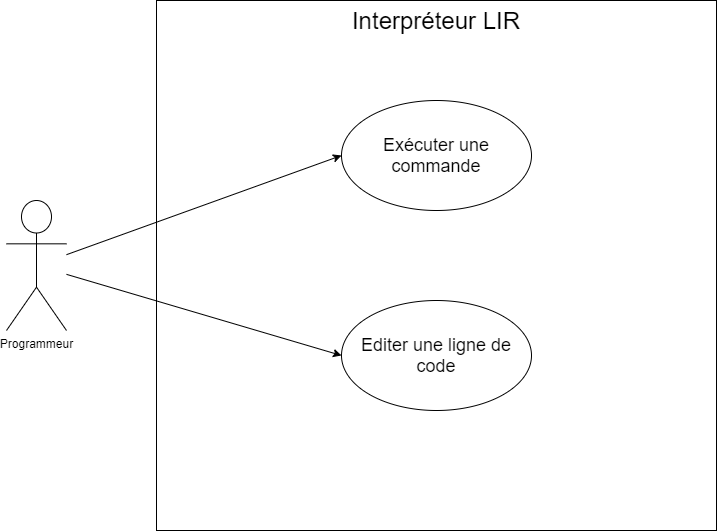
\includegraphics[width=\linewidth]{img/DiagrammeCasUtilisation.png}

    \subsection{Les acteurs}
    \paragraph{Programmeur :} % TODO à détailler
    Personne utilisant l'interpréteur.

    \subsection{Résumés de cas d'utilisation}
    \subsubsection{\Large --- Exécuter une commande}

        \subparagraph{Acteurs}
    Programmeur : il entre une commande à faire exécuter immédiatement par l'interpréteur.

    \subparagraph{Objectifs}
    Exécuter la commande entrée dans l'interpréteur.

    \subparagraph{Pré-Conditions}
    L'interpréteur LIR est lancé et le curseur est derrière l'invite.

    \subparagraph{Post-Conditions}
    La commande est exécutée et un résultat ou un feedback est affiché.

    \subparagraph{Scénario nominal (grandes étapes)}
        \begin{enumerate}
            \item Le programmeur écrit derrière l'invite une ligne de commande.
            \item Le programmeur valide cette commande.
            \item L'interpréteur effectue une analyse lexico-syntaxique.
            \item L'interpréteur interprète la ligne de commande.
        \end{enumerate}

    \subparagraph{Scénarios d'échec}
        \subparagraph{Point 3 du scénario nominal :} la syntaxe de la ligne écrite est incorrecte.
        \begin{itemize}
            \item Un message d'erreur explicite informe le programmeur.
            \item Retour au point 4 du scénario nominal.
        \end{itemize}

        \subparagraph{Point 4 du scénario nominal :} la commande conduit à une erreur d'exécution.
        \begin{itemize}
            \item Un message d'erreur explicite informe le programmeur.
            \item Retour au point 4 du scénario nominal.
        \end{itemize}

%\end{document}

    \subsubsection{\Large --- Éditer une ligne de code}

    
\title{Résumé de cas d'utilisation --- Éditer une ligne de code} % à remplacer


        \subparagraph{Acteurs}
            Programmeur : Il écrit ou modifie une ligne de code dans un
            programme à faire exécuter par l'interpréteur.

        \subparagraph{Objectifs}
            Écrire une une ligne de code dans nouveau programme ou un
            existant afin d'exécuter ou de sauvegarder ce programme.

        \subparagraph{Pré-conditions}
                Le curseur est derrière l'invite suivi d'une étiquette correspondant
                au numéro de la ligne de code à éditer.

        \subparagraph{Post-conditions}
                Le code source édité est prêt à être exécuté, abandonné ou sauvegardé,
                selon l'intention du programmeur.

        \subparagraph{Scénario nominal (grandes étapes)}
            \begin{enumerate}
                \item Le programmeur écrit une instruction ou commande par ligne de code, en la faisant précéder de son étiquette.

                \item Le programmeur consulte le code déjà écrit à tout moment avec la
                      commande \verb|liste|. Selon la syntaxe choisie, l'interpréteur
                      affiche la plage demandée ou la totalité des lignes de code
                      du programme dans l'ordre croissant des étiquettes.

                \item Le programmeur consulte la liste des identificateurs déclarés et
                      leurs valeurs en entrant la commande \verb|defs|.

                \item Au besoin, le programmeur efface une ou plusieurs lignes avec la
                      commande \verb|efface|.

                \item Au besoin, le programmeur efface les lignes de code et identificateurs mémorisés et commence un nouveau code avec la commande \verb|debut|.
            \end{enumerate}

        \subparagraph{Scénarios d'échec}

            \paragraph{Point 2 du scénario nominal :} Aucune ligne de code n'est écrite ou
            la plage de code à afficher n'est pas correcte.
            \begin{itemize}
                \item L'interpréteur en avise le programmeur au moyen d'un message d'erreur.
                \item Retour au point 1.
            \end{itemize}

            \paragraph{Point 3 du scénario nominal :} Aucun identificateur n'a encore été
            déclaré.
            \begin{itemize}
                \item L'interpréteur affiche un message informant le programmeur.
                \item Retour au point 1.
            \end{itemize}

            \paragraph{Point 4 du scénario nominal :} La plage de ligne à effacer est
            incorrecte.
            \begin{itemize}
                \item Un message d'erreur en informe le programmeur
                \item Retour au point 1.
            \end{itemize}


    \subsection{Récits d'utilisation (user stories)}
    Les récits d'utilisation %TODO déf
    \\Des récits d'utilisation ont été rédigés pour chaque commande et instruction.


    \chapter{Organisation du projet}
    \section{Présentation du cycle de vie itératif} % TODO relecture
    Pour développer l’Interpréteur LIR, le modèle de cycle de vie itératif a été
    choisi. Ce modèle de développement de logiciel consiste en une succession de
    cycles de spécification, de conception, de réalisation et de tests, le but
    est d’enrichir et de « remodeler » des prototypes du logiciel successifs. Par
    conséquent, une version du logiciel sera un « dernier prototype ».
    \\La gestion du risque va entraîner la mise en place d’un noyau architectural
    avec des fonctions indispensables du logiciel dès les deux premières
    itérations. Les itérations suivantes apporteront des corrections et de
    nouvelles fonctions au logiciel.
    \\Les versions successives des prototypes permettent de matérialiser
    l’avancement et d’éviter « l’effet tunnel » sur le projet. Ces prototypes
    (versions 0.x) entretiennent la motivation des différents acteurs du projet :
    l’équipe MOE, la MOA.
    \\Le principe fondamental à chaque début d’itération est de ne spécifier en
    détail que les fonctionnalités nécessaires pour cette itération. Ainsi la
    prise en compte d’évolutions du besoin reste possible jusqu'à la dernière
    itération. De même le « refactoring » de la conception (largement facilité
    par les outils) a lieu à chaque étape pour intégrer des évolutions et des
    ajouts. Le but étant bien sûr de fabriquer le logiciel adapté au besoin en
    laissant la possibilité de « mûrir » au cours du temps.
    \\Ce type de cycle implique une taille homogène de l’équipe et une
    polyvalence des équipiers.

    \section{Répartition des rôles}
    Rôles des membres de l’équipe impliqués dans le projet jusqu'au mois de mai
    2021 :
    \begin{center}
        \begin{tabular}{rl}
            Chef de projet MOE            & Pierre Debas      \\
            Secrétaire de projet          & Heïa Dexter       \\
            Gestionnaire de configuration & Sylvan Courtiol   \\
            Développeur                   & Nicolas Caminade  \\
            Développeur                   & Lucàs Vabre       \\
        \end{tabular}
    \end{center}

    \section{Plan communication}
    \subsection{Localisation géographique des intervenants}
    L'équipe MOE, la MOA et les contrôleurs qualités sont basés sur Rodez (12).
    \\La MOA, les contrôleurs qualités, H. Dexter sont basés sur Rodez (12), S.
    Courtiol sur Luc-La-Primaube à côté de Rodez (12), P. Debas est basé à la
    fois sur Rodez et à Albi (81), L. Vabre sur Gages (12) et N. Caminade sur
    Rodez et Moncaut (47).

    \subsection{Moyens de communication utilisés}
    Les communications formelles sont effectuées via les mails de l’IUT
    (généralement par le chef de projet) avec les autres membres du projet en CC.
    \\Serveur Discord spécifique au projet pour communication écrite ou vocale de
    la MOE.
    \\Cf. le document Configuration interpréteur du langage LIR produit par le
    gestionnaire de configuration (S. Courtiol).

    \subsection{Réunions projets MOE}
    Les réunions projet MOE seront hebdomadaires voire bi-hebdomadaires et dans
    le contexte de la crise sanitaire elles se dérouleront en distanciel via
    Discord (vocal, visio-conférence). Seront prévue des réunions courtes de 20
    minutes et des réunions longues de 1h30.
    \\Ces réunions auront pour objectif de faire le point sur l’avancement du
    projet, le respect des objectifs fixé sur la période et de fixer les
    prochains objectifs à remplir d’ici la prochaine réunions. Aussi ces réunions
    seront l’occasion de faire part de difficultés éventuelles rencontrées par
    les membres de l’équipe au cours de la semaine et de communiquer les
    informations sur les prochaines rencontres avec la MOA.
    \\Les comptes-rendus seront rédigés par la secrétaire de projet (H. Dexter)
    et diffusés sur le serveur Discord de l’équipe sous format texte.

    \subsection{Comités de Pilotage}
    Les comités de pilotage rassembleront la MOA et toute l’équipe de MOE. Les
    COPIL seront dirigé par le chef de projet éventuellement assisté par le
    secrétaire.
    \\La fréquence des COPIL est au mieux hebdomadaire et d’une durée d’une
    demi-heure à trois quarts d’heure selon l’avancement du projet.
    Les comptes-rendus des COPIL seront rédigés par l’actuelle secrétaire de
    projet (H. Dexter) et diffusés le lendemain à la MOE du projet.


    \section{Assurance qualité}
    \subsection{Normes et standards de travail à observer (formalisme de modélisation, méthodes de contrôle, méthodes de développement, cycle de vie, conventions de code…)}
    Pour mener à bien ce projet l'équipe MOE travaille
    en utilisant le langage UML comme formalisme de modélisation, la méthode de
    développement dirigé par les tests i.e. la méthode TDD (Test Driven
    Development) en respectant les Java Code Convention pour un modèle de cycle
    de vie itératif.

    \subsection{Manuel qualité et démarche qualité à observer (suivant la politique qualité de l’organisation), suivi et contrôle qualité (organisation, fréquence, participants).}
    % TODO: À commencer


    \section{Ressources matérielles et logicielles}
    % principaux matériels, réseaux, systèmes d’exploitation, sites intranet-internet (wiki, gestionnaire d’incident, référentiel…) et outils de génie logiciel utilisés.

    % TODO: ajouter le doc de Sylvan

    \chapter{Pilotage du projet}
    \section{Cycle de vie itératif}
    Pour développer l’Interpréteur LIR, le modèle de cycle de vie itératif a été
    choisi. Ce modèle de développement de logiciel, rappelons-le, consiste en une
    succession de cycles de spécification, de conception, de réalisation et de
    tests, le but est d’enrichir et de « remodeler » des prototypes du logiciel
    successifs. Par conséquent, une version du logiciel sera un « dernier
    prototype ».
    \\Si le choix de modèle de cycle de vie s'est porté sur le modèle itératif,
    c'est parce qu'il s'agit d'un modèle "réaliste" et possible à mettre en place
    dans le cadre des projets tuteurés :

    \begin{itemize}
        \item Une limitation de "l'effet tunnel" pour une meilleure dynamique et motivation des équipes (MOA et MOE).
        \item Une meilleure acceptation des changements grâce aux prototypes.
        \item Une meilleure gestion des risques.
        \item Est adapté pour une équipe de cinq personnes polyvalentes.
        \item Le principe d'itérations où seules les fonctionnalités nécessaires sont spécifiées en détail en début d'itération ce qui permet une évolution du besoin.
    \end{itemize}

    \section{Estimation initiale}
    \section{Planification prévisionnelle initiale}
    \section{Durée et ordonnancement des principales tâches et itérations}
    \section{Identification des premiers jalons}
    \section{Calendrier prévisionnel}
    \section{Organisation des réunions projets et comités de pilotage}
    \section{Suivi du projet par période}
    Pour chaque période :
    \subsection{Suivi d’avancement et mesure des écarts par rapport au prévisionnel revu lors de la période précédente}

    \subsection{Synthèse par "tableau de bord"}

    \subsection{Résultats des tests et recette de prototype de la période}

    \subsection{Résultats des revues/suivis/contrôles qualité de la période}

    \subsection{Identification des principaux écarts et problèmes constatés, solutions possibles}

    \subsection{Propositions de modification de la planification prévisionnelle pour tenir compte des corrections à apporter}

    \subsection{Comptes-rendus des réunions projets de la période}

    \subsection{Compte-rendu du comité de pilotage de la période}

    \subsection{Planification prévisionnelle révisée pour les périodes suivantes (en fonction des décisions prises)}


    % TODO: Glossaire


    \part{Annexes}

    \appendix
    %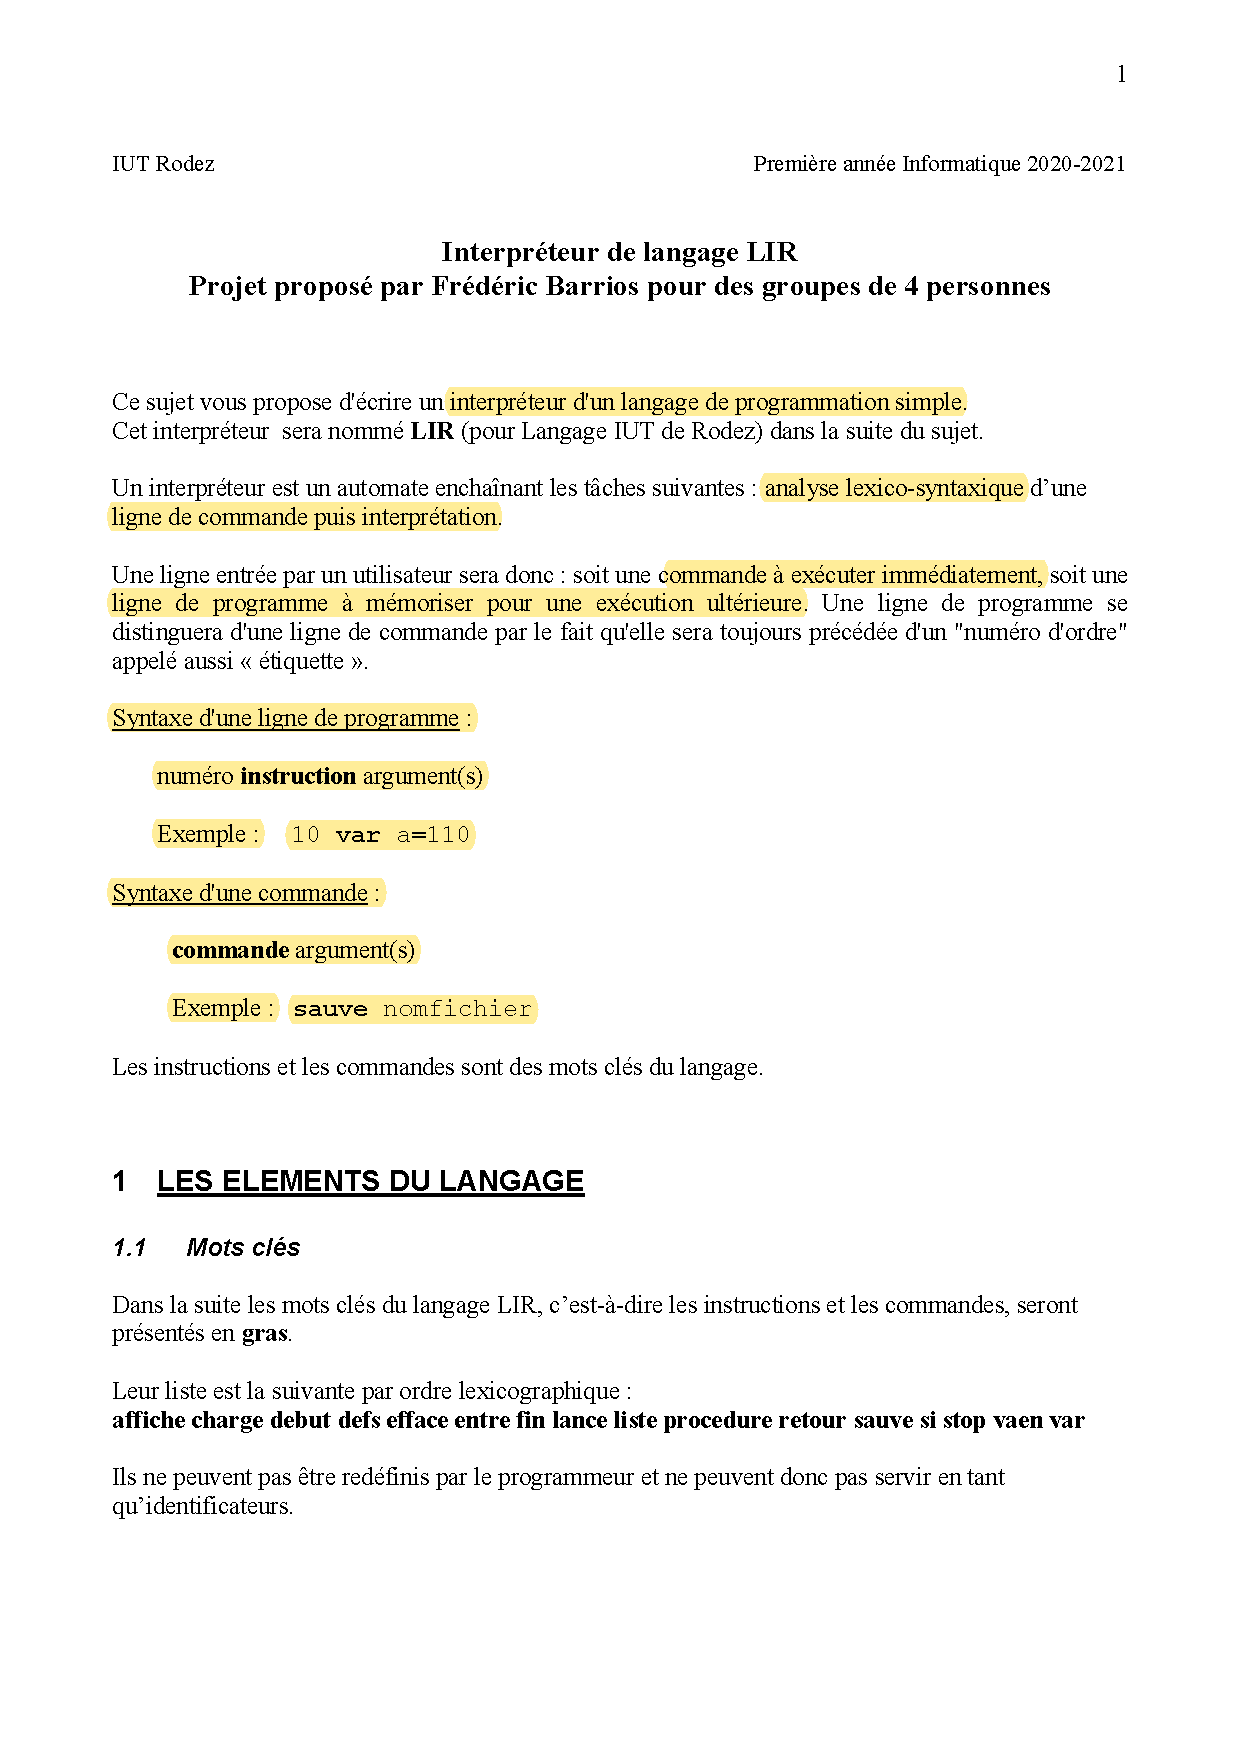
\includepdf[pages=-]{fichiers/BarriosInterpreteurLIR2021}
    \chapter{Sujet Interpréteur LIR}

    \documentclass[11pt,a4paper,titlepage,openright]{report}
\usepackage[utf8]{inputenc}
\usepackage[T1]{fontenc}
\usepackage[french]{babel}
\usepackage[top=1.5cm, bottom=5cm]{geometry}
\usepackage{fancyhdr, graphicx, array, hyperref}
\usepackage{glossaries}

\pagestyle{fancy}

\title{\textsc{\textbf{Gestion de la configuration\\Interpréteur du langage LIR}}}
\date{}
\author{Nicolas \textsc{Caminade} \and Sylvan \textsc{Courtiol} \and Pierre \textsc{Debas} \and Heïa \textsc{Dexter} \and Lucàs \textsc{Vabre} }
\begin{document}
    \lhead{Gestion de la configuration}
    \rhead{
        
\includegraphics[width=2cm]{img/logoiut}
    }

    \cfoot{\thepage}
    \headheight = 2cm
    \headsep = 1.5cm


    \begin{titlepage}
        \fontfamily{pag}\selectfont

        \begin{center}\normalsize
            \MakeUppercase{IUT de Rodez \hfill Département informatique \hfill INFO1 2020-2021}
        \end{center}
        \vspace*{0.1cm}
        \hrule
        \vspace*{0.2cm}
        \begin{flushright}
            
\includegraphics[width=4cm]{img/logoiut}
        \end{flushright}
        \vspace*{2cm}
        \begin{flushright}\Huge
            \textsc{\textbf{Gestion de la configuration\\Interpréteur du langage LIR}}
        \end{flushright}
        \hrule
        \begin{flushleft}
            \MakeUppercase{Projet proposé par Frédérique Barrios}
        \end{flushleft}
        \vspace*{1cm}
        \begin{center}\normalsize
        	\textbf{version : \today}
        \end{center}
        \vspace*{1cm}
        \begin{center}\Large
            Nicolas \textsc{Caminade}, Sylvan \textsc{Courtiol},\\
            Pierre \textsc{Debas}, Heïa \textsc{Dexter}, \\
            Lucàs \textsc{Vabre}
        \end{center}
        \vfill
        \begin{center}\normalsize
            \MakeUppercase{Projet tuteuré --- Semestre 2}
        \end{center}
    \end{titlepage}


    % Sommaire
    \renewcommand{\contentsname}{Sommaire}
    \tableofcontents
    
    \newpage

    % numérotation des sections et sous-section indiféremment des chapitres
    \setcounter{section}{0}
    \renewcommand{\thesection}{\arabic{section}} 
    \renewcommand{\thesubsection}{\arabic{section}.\arabic{subsection}}
    
    
    \section*{Introduction}
    \Large
    Ce document a pour but de confirmer par écrit la configuration logicielle choisie pour le
    projet.
    \par Le contenu de ce document n’est pas fixé et des changements peuvent être apportés. Cependant ce document doit être connu et suivi par les membres du groupe. En cas de modifications, une annonce sur discord sera faite.
    \par Pour toute question ou suggestion se référer au gestionnaire de configuration (présentement
    Sylvan COURTIOL).


    \normalsize
    \section{Logiciels de développement}
        \subsection{Environnement de Développement Intégré}
        Eclipse JEE (version 2020-12)
        \par JDK 15
        
        \subsection{Contrôle des versions du code}
        Git (notamment intégré à Eclipse) avec dépôt sur GitHub. (Un apprentissage est nécessaire
        donc pour commencer certaines libertés sont possibles).
        
        \subsection{Organisation}
        Via le site Trello (non utilisé pour le moment).
        
    \section{Logiciels généraux}
        \subsection{Communication}
        \par Les communications formelles sont effectuées via les mails de l’IUT (généralement par le chef
        de projet) avec les autres membres du projet en CC.

        \par Serveur discord spécifique au projet pour la communication écrite ou vocale de la MOE.
        \par Google Meet pour les réunions avec les personnes autres que MOE. Adaptable à ce qui
        convient le mieux à cette personne.
        
        \subsection{Éditeur de texte}
        Le traitement de texte sera fait sous LaTex notamment avec la distribution MiKTex et l'IDE TexStudio. Les documents texte sont partagés en PDF ou version papier à la MOA/MOE  et en format modifiable .tex seulement à la MOE via la solution de partage distant des fichiers (voir sous-section suivante).
        
        \subsection{Partage distant des fichiers}
        Les partages de tous les fichiers généraux et codes sources se feront sur GitHub via le site, le logiciel GitHub desktop ou git. Il y aura également une intégration Discord informant des commits.
        
    \section{Sécurité}
    \par Si possible tous les membres du groupe auront les mêmes droits sur les fichiers communs.
    En conséquence aucun membre du groupe ne doit donner des droits sur ces fichiers à une
    personne extérieure au projet (autre que MOA).
    \par Les sauvegardes du dépôt GitHub (contenant toutes les données du projets) seront effectuées
    régulièrement (tous les 1 ou 2 jours) par le gestionnaire de configuration. Toutes données qui ne
    sont pas dans le dépôt sont à la responsabilité de chacun.
    Les sauvegardes sont enregistrée en local par le gestionnaire de configuration ainsi que sur le Google drive partagé du projet.



    \appendix
    %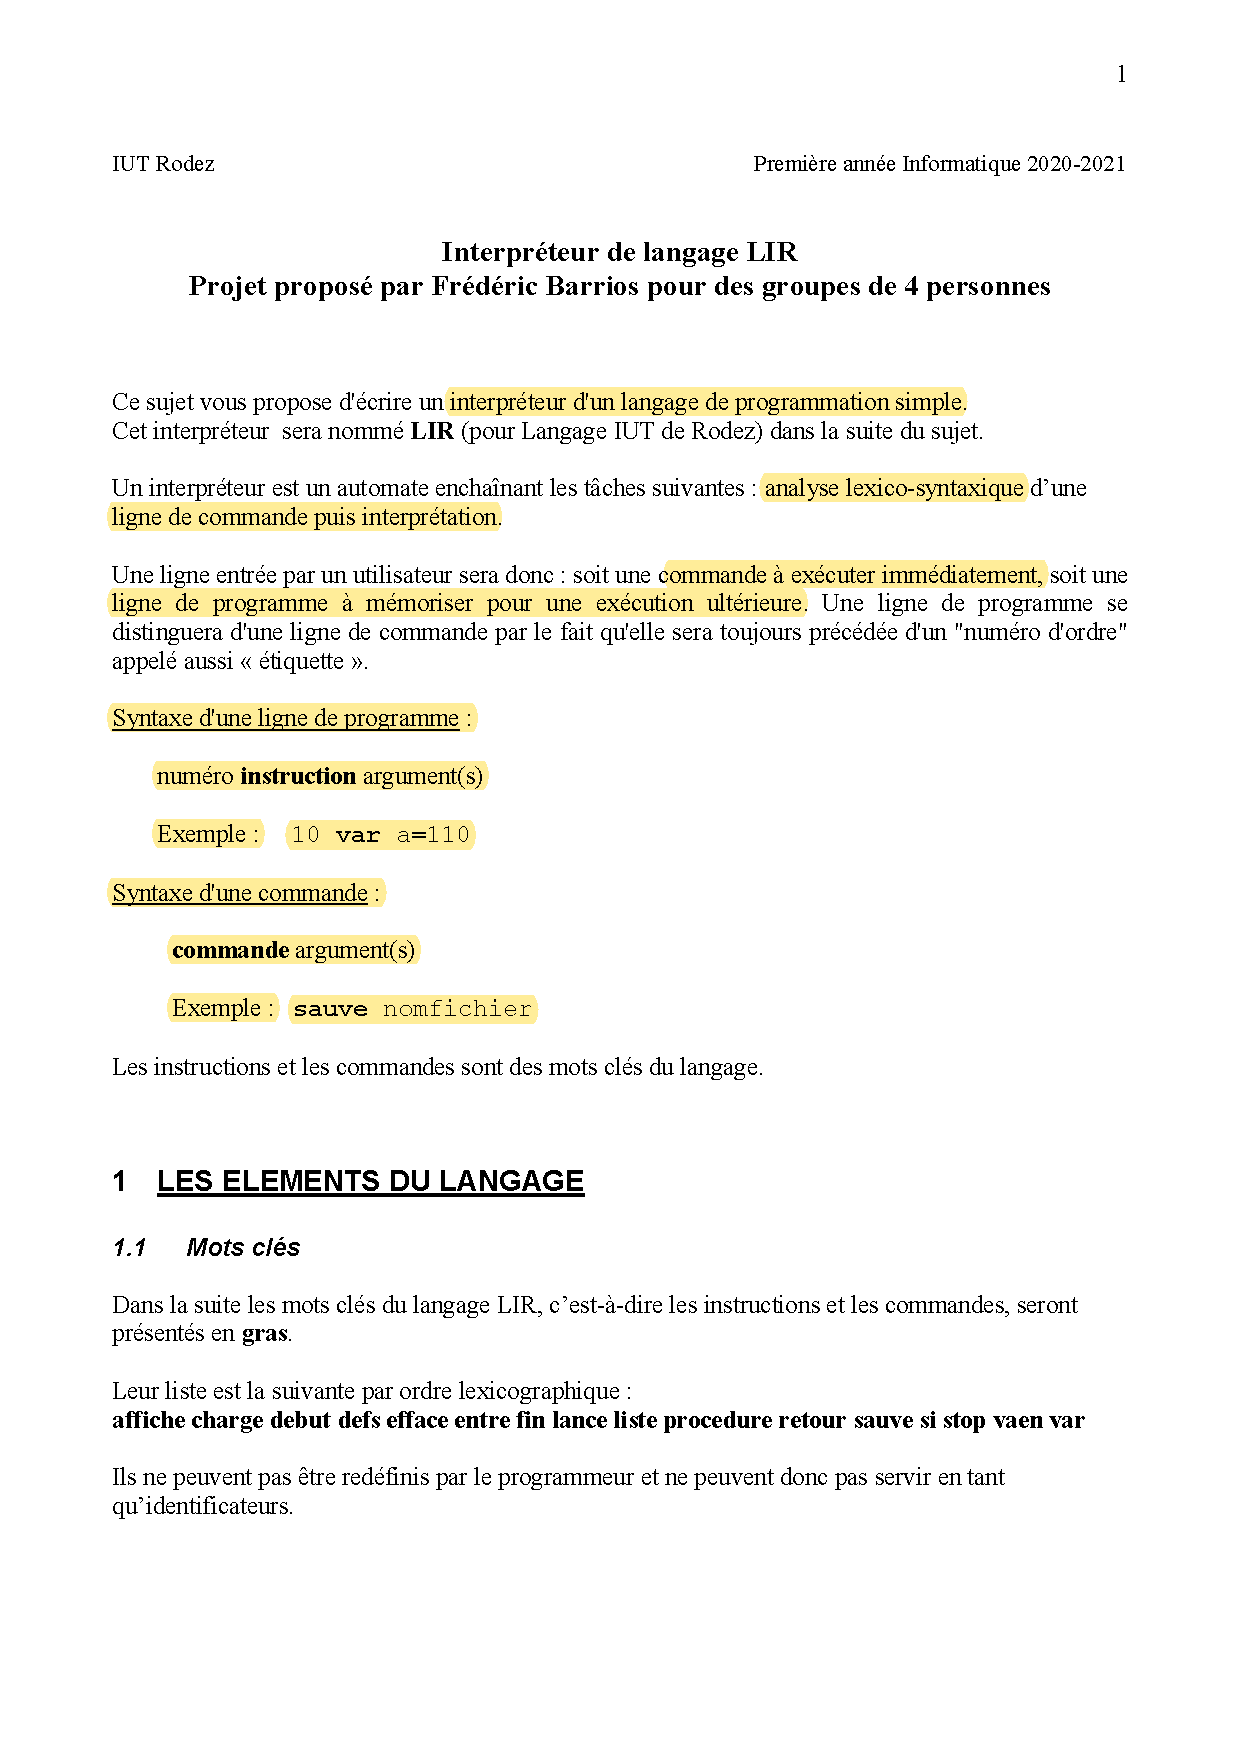
\includepdf[pages=-]{fichiers/BarriosInterpreteurLIR2021}

\end{document}
    \pagestyle{fancy}

\title{\textsc{\textbf{Étude du besoin --- Récits d'utilisation
                       \\Interpréteur du langage LIR}}}
\date{}
\author{Nicolas \textsc{Caminade} \and Sylvan \textsc{Courtiol} \and
    Pierre \textsc{Debas} \and Heïa \textsc{Dexter} \and Lucàs
    \textsc{Vabre} }
%\begin{document}
    \lhead{\leftmark}
    \rhead{
        
\includegraphics[width=2cm]{./img/logoiut}
    }

    \cfoot{\thepage}
    \headheight = 2cm
    \headsep = 0.5cm

    \begin{titlepage}
        \fontfamily{pag}\selectfont

        \begin{center}\normalsize
            \MakeUppercase{IUT de Rodez \hfill Département informatique
                \hfill INFO1 2020-2021}
        \end{center}
        \vspace*{0.1cm}
        \hrule
        \vspace*{0.2cm}
        \begin{flushright}
            
\includegraphics[width=4cm]{./img/logoiut}
        \end{flushright}
        \vspace*{2cm}
        \begin{flushright}\Huge
            \textsc{\textbf{Etude du besoin \\ Récits d'utilisation
                    \\Interpréteur du langage LIR}}
        \end{flushright}
        \hrule
        \begin{flushleft}
            \MakeUppercase{Projet proposé par Frédérique Barrios}
        \end{flushleft}
        \vspace*{2cm}
        \begin{center}\Large
            Nicolas \textsc{Caminade}, Sylvan \textsc{Courtiol},\\
            Pierre \textsc{Debas}, Heïa \textsc{Dexter}, \\
            Lucàs \textsc{Vabre}
        \end{center}
        \vfill
        \begin{center}\normalsize
            \MakeUppercase{Projet tuteuré --- Semestre 2}
        \end{center}
    \end{titlepage}

    \chapter{Récits d'utilisation de l'Interpréteur LIR}

    \Large
    Texte. Blablabla

    \chapter*{Récits d'utilisation proposés lors de l'itération 1}

        \section{Commande}

    \subsection*{Récit d'utilisation}

    \paragraph{Titre : } Exécution d'une commande
        \paragraph{Récit : } Exécution d'une commande
    \paragraph{En tant que : } programmeur avec l'interpréteur LIR
    \paragraph{Je souhaite : } exécuter une commande
    \paragraph{Afin de : } obtenir le résultat de cette commande ou une
                               confirmation de son exécution
    \subsection*{Critères d'acceptation}

    \paragraph{À partir du fait : } l'interpréteur affiche un invite
    \paragraph{Alors : } j'entre une ligne de commande
    \paragraph{Enfin : } j'obtiens le résultat de cette commande ou un retour
    m'informant du bon déroulé de l'exécution de la commande ou de son échec.
    \newpage
        \section{Commande debut}
    \subsection*{Récit d'utilisation}

    \paragraph{Titre : } debut
    \paragraph{Récit : } Réinitialiser l'environnement de l'interpréteur LIR
    \paragraph{En tant que : } programmeur
    \paragraph{Je souhaite : } vider l'intégralité du contexte d'exécution
    \paragraph{Afin de : } obtenir un environnement de travail vierge

    \subsection*{Critères d'acceptation}

    \paragraph{À partir de : } d'une session de l'interpréteur LIR
    \paragraph{Alors : } j'entre la commande \verb|debut|
    \paragraph{Enfin : } L'interpréteur efface toutes les lignes de programme
    mémorisées ainsi que tous les identificateurs mémorisés
    \newpage
        \section{Commande fin}

    \subsection*{Récit d'utilisation}

    \paragraph{Titre : } Quitter l'interpréteur (commande fin)
    \paragraph{Récit : } Quitter l'interpréteur (commande fin)
    \paragraph{En tant que : } programmeur avec l'interpréteur LIR
    \paragraph{Je souhaite : } quitter l'interpréteur
    \paragraph{Afin de : } arrêter d'utiliser l'interpréteur LIR pour la session courante

    \subsection*{Critères d'acceptation}

    \paragraph{À partir du fait : } je suis en train d'utiliser l'interpréteur
    \paragraph{Alors : } je souhaite quitter l'interpréteur pour la session courante en exécutant la commande fin
    \paragraph{Enfin : } le processus courant de l'interpréteur LIR s'arrête
    \newpage
        \section{Commande defs}
    \subsection*{Récit d'utilisation}

    \paragraph{Titre : } Affichages du contexte courant (commande defs) % Écrire le titre à la place du commentaire
    \paragraph{Récit : } Affichages du contexte courant (commande defs) % Écrire nom du récit à la suite
    \paragraph{En tant que : } programmeur avec l'interpréteur LIR % Remplacer commentaire par rôle
    \paragraph{Je souhaite : } voir toutes les variables définies dans la session courante (identificateur et valeur)
    \paragraph{Afin de : } connaître le contexte actuel de la session courante de l'interpréteur

    \subsection*{Critères d'acceptation}

    \paragraph{À partir du fait : } des variables sont définies dans la session courante de l'interpréteur
    \paragraph{Alors : } je souhaite connaître le contexte actuel en exécutant la commande defs
    \paragraph{Enfin : } l'interpréteur affiche chaque variable ligne par ligne avec son identificateur et sa valeur

    \newpage
        \section{Commande affiche}

	\subsection*{Récit d'utilisation}

	\paragraph{Titre : } Faire un saut de ligne avec la commande affiche
	\paragraph{Récit : }  Provoquer le saut de ligne sur la sortie de texte courante
	\paragraph{En tant que : } Programmeur
	\paragraph{Je souhaite : } que l'interpréteur LIR saute une ligne sur la sortie de texte courante
	\paragraph{Afin de : } Provoquer un saut de ligne sur cette sortie

	\subsection*{Critères d'acceptation}

	\paragraph{À partir du fait : } que j'ai une sortie de texte courante
	\paragraph{Alors : } j'entre la commande affiche
	\paragraph{Enfin : } l'interpréteur saute une ligne sur la sortie de texte courante
    \newpage
        \section{Commande affiche avec une expression}

	\subsection*{Récit d'utilisation}

	\paragraph{Titre : } Commande affiche (expression)
	\paragraph{Récit : }  Afficher le contenu d'une expression sur la console de l'interpréteur
	\paragraph{En tant que : } Programmeur
	\paragraph{Je souhaite : } que l'interpréteur LIR évalue et affiche le contenu de l'expression que l'on lui donne
	\paragraph{Afin de : } pouvoir récupérer/vérifier le/les résultat(s) de son programme

	\subsection*{Critères d'acceptation}

	\paragraph{À partir du fait : } que j'ai la possibilité de saisir une ligne de commande
	\paragraph{Alors : } je tape la commande affiche et écrit l'expression dont je veut que la valeur soit affichée à la suite : affiche <expression>
	\paragraph{Enfin : } l'interpréteur évalue dans l'expression spécifiée la valeur de celle-ci et renvoie cette valeur sur la console et affiche un résultat sur LIR (en tant que feed-back) pour nous spécifier si la commande a bien pu s'exécuter

    \newpage
        \section{Commande var pour une chaîne de caractères}

    \subsection*{Récit d'utilisation}

    \paragraph{Titre : } Commande var (Chaine de caractères)
    \paragraph{Récit : }  Initialiser une chaine de caractère dans variable / Changer sa valeur
    \paragraph{En tant que : } Programmeur
    \paragraph{Je souhaite : } que l'interpréteur LIR stock une chaine dans une variable
    \paragraph{Afin de : } pouvoir récupérer/manipuler cette chaine plus tard dans le programme


    \subsection*{Critères d'acceptation}

    \paragraph{À partir du fait : } que j'ai la possibilité de saisir une ligne de commande
    \paragraph{Alors : } je tape la commande var et met une chaine de caractère entre double guillements comme valeur : var <nomVariable>="<chaine>"
    \paragraph{Enfin : } l'interpréteur enregistre dans la variable spécifié la chaine de caractère voulue et renvoie la variable suivie de sa valeur (en tant que feed-back)
    \newpage
        \section{Commande var pour un entier}
   \subsection*{Récit d'utilisation}

    \paragraph{Titre : } Commande var (Entier)
    \paragraph{Récit : }  Initialiser un entier dans variable / Changer sa valeur
    \paragraph{En tant que : } Programmeur
    \paragraph{Je souhaite : } que l'interpréteur LIR stock un entier dans une variable
    \paragraph{Afin de : } pouvoir récupérer/manipuler cet entier plus tard dans le programme

    \subsection*{Critères d'acceptation}

    \paragraph{À partir du fait : } que j'ai la possibilité de saisir une ligne de commande
    \paragraph{Alors : } je tape la commande var et met un entier comme valeur :
    \verb |var <nomVariable>=<entier> |
    \paragraph{Enfin : } l'interpréteur enregistre dans la variable spécifié l'entier voulu et renvoie la variable suivie de sa valeur (en tant que feed-back)

    \newpage
        \section{Expression concaténation sur chaîne de caractères}

    \subsection*{Récit d'utilisation}

    \paragraph{Titre : } Opérateur + sur les chaînes de caractères
    \paragraph{Récit : } Concaténation de chaînes
    \paragraph{En tant que : } Programmeur
    \paragraph{Je souhaite : } accoler deux chaînes l'une à la suite de l'autre
    \paragraph{Afin de : } créer des messages dépendant du contexte d'exécution sur
    la sortie standard. Représenter une valeur entière par son écriture chiffrée en
    base 10.


    \subsection*{Critères d'acceptation}

    \paragraph{À partir de : } deux chaînes de caractères ou une chaîne et un entier,
    en tant qu'identificateurs déclarés ou expressions littérales.

    \paragraph{Alors : } En utilisant une expression de type
    \verb|var nouvelleChaine = opeGauche + opeDroite|, j'obtiens la concaténation de
    deux chaînes.

    \paragraph{Enfin : } L'identificateur \verb|nouvelleChaine| contient la chaîne
    constituée des deux primordiales concaténées. L'interpréteur confirme en affichant
    la nouvelle valeur ou m'informe d'une erreur. L'opération peut être récursive mais n'est pas commutative. Une concaténation s'effectue toujours par la droite.
    \newpage
        \section{Expression logique}

    \subsection*{Récit d'utilisation}

    \paragraph{Titre : } Expression logique dans un branchement
    conditionnel
    \paragraph{Récit : } Opérations relationnelles sur deux entiers
    \paragraph{En tant que : } Programmeur
    \paragraph{Je souhaite : } que l'Interpréteur LIR compare deux
    entiers avec une relation d'ordre ou d'équivalence
    \paragraph{Afin que : } d'exécuter ou non une branche du code avec
    l'instruction si

    \subsection*{Critères d'acceptation}

    \paragraph{À partir de : } d'une ligne de programme à mémoriser et d'identificateurs auxquels une valeur aura été affectée préalablement
    ou de constantes littérales de type entier signé.

    \paragraph{Alors : } j'entre une expression composée de deux
    opérandes de type entier signé et d'un opérateur et l'interpréteur
    évalue l'expression.
    \\ Les opérandes peuvent être :
    \begin{itemize}
        \item deux constantes littérales
        \item deux identificateurs
        \item une constante littérale et un identificateur
    \end{itemize}

    \paragraph{Enfin : } si l'expression (condition dans l'instruction)
    est vraie alors l'exécution continuera à partir du numéro de ligne
    spécifié par l’étiquette, sinon l'exécution continuera en séquence.
    \newpage
    \documentclass[12pt,a5paper, notitle, oneside]{report}
\usepackage[utf8]{inputenc}
\usepackage[T1]{fontenc}
\usepackage[french]{babel}
\usepackage[landscape, top=0.5cm]{geometry}
\begin{document}

    \chapter*{Récit d'utilisation}

    \paragraph{Titre : } Expression arithmétique
    \paragraph{Récit : } Calcul à l'aide d'expression arithmétique
    \paragraph{En tant que : } Programmeur
    \paragraph{Je souhaite : } que l'Interpréteur LIR effectue une
    opération arithmétique courante (addition, soustraction,
    multiplication, quotient ou reste d'une division entière)
    \paragraph{Afin que : } j'en exploite ou vois le résultat
    \newpage

    \chapter*{Critères d'acceptation}

    \paragraph{À partir de : } d'une ligne de l'interpréteur ou d'une
    ligne de programme à mémoriser et d'identificateurs auxquels une
    valeur aura été affectée préalablement ou de constantes littérales
    numérique.

    \paragraph{Alors : } j'entre une expression composée de deux
    opérandes de type entier signé et d'un opérateur.
    \\ Les opérandes peuvent être :
    \begin{itemize}
        \item deux constantes littérales
        \item deux identificateurs
        \item une constante littérale et un identificateur
    \end{itemize}
    \paragraph{Enfin : } j'obtiens le résultat de l'opération ou un
    message d'erreur m'informant que l'opération est impossible pour les
    identificateurs ou constantes littérales saisies.

\end{document}

    \chapter*{Récits d'utilisation proposés lors de l'itération 2}


\end{document}